\documentclass[a4paper,12pt]{article} % тип документа
%  Русский язык
\usepackage{multirow}
\usepackage{wrapfig}
\usepackage[T2A]{fontenc}			% кодировка
\usepackage[utf8]{inputenc}			% кодировка исходного текста
\usepackage[english,russian]{babel}	% локализация и переносы

\usepackage{indentfirst} %Красная строка
\usepackage[a4paper,top=1.3cm,bottom=2cm,left=1.0cm,right=1.5cm,marginparwidth=0.75cm]{geometry}
\usepackage[usenames]{color}
\usepackage{colortbl}
\usepackage{float}

\usepackage{graphicx}%картинки
\usepackage{wrapfig}%обтекание текстом таблиц и картинок
%гиперссылки
\usepackage{hyperref}
\usepackage[rgb]{xcolor}
\hypersetup{     %гипперсылки
 colorlinks=true, %false:ссылки в рамках
 urlcolor=blue   %на URL
 }
% Заметки
\usepackage{todonotes}

% Математика
\usepackage{amsmath,amsfonts,amssymb,amsthm,mathtools} 
\usepackage{hyperref}
\renewcommand{\baselinestretch}{1.5}

\begin{document}

\begin{titlepage}
\begin{center}
    {\large МОСКОВСКИЙ ФИЗИКО-ТЕХНИЧЕСКИЙ ИНСТИТУТ (НАЦИОНАЛЬНЫЙ ИССЛЕДОВАТЕЛЬСКИЙ УНИВЕРСИТЕТ)}
\end{center}

\begin{center}
    {\large Физтех-школа аэрокосмических технологий}
\end{center}
	\hfill \break
	\hfill\break
	\hfill\break
	\hfill \break
	\hfill \break
	\hfill \break
	\hfill \break
	\hfill \break
	\hfill \break
\begin{center}
    {\bf Лабораторная работа по оптике 4.3.1:}\\
    {\bf Изучение дифракции света}\\
    Выполнила: Ефимова Арина, Б03-106.
\end{center}
\end{titlepage}

\begin{center}
    {\large Изучение дифракции света}
\end{center}

\textbf{Цель работы:} Исследовать явление дифракции Френеля и Фраунгофера на щели, изучить влияние дифракции на разрешающую способоность оптических инструментов. \\

\textbf{В работе используются:} оптическая скамья, ртутная лампа, моно хроматор, двойная щель, микроскоп на поперечных слазках с микрометрическим винтом, зрительная труба.\\




\section{Теоретическая справка}
\subsection*{А. Дифракция Френеля}
\begin{figure}[h]
\includegraphics[scale=0.7]{0.png}
\centering
\caption{\label{fig:first}Схема установки 1.}
\end{figure}
Схема установки представлена на Рис. \ref{fig:first}. Световые лучи освещают щель $S_2$ и испытывают на ней дифракцию. Дифракционная картина рассматривается с помощью микроскопа М, сфокусированного на некоторую плоскость наблюдения П. Щель $S_2$ освещается параллельным пучком монохроматического света с помощью коллиматора, образованного объективом $O_1$ и щелью $S_1$, находящейся в его фокусе. На $S_1$ сфокусированно изображение спектральной линии, выделенной из спектра ртутной лампы Л при помощи монохроматор $C$, в котором используется призма прямого зрения. \\
Распределение интенсивности света в плоскости П рассчитаем с помощью зон Френеля. При освещении $S_2$ параллельным пучком лучей (плоская зона) зоны Френеля представляют собой плоскости, параллельные краям щели. Результирующая амплитуда в точке наблюдения определеяется суперпозицией колебаний от тех зон Френеля, которые не перекрыты створками щели. Графическое определение результирующей амплитуды производится с помощью векторной диаграммы -- спирали Корню. Суммарная ширина $m$ зон Френеля $\xi_m$ определяется соотношение
\begin{equation}
\xi_m = \sqrt{am\lambda},
\end{equation}
где $a$ -- расстояние от щели до плоскости П. Вид наблюдаемой картины определяется \textit{числом Френеля} $\Phi$:
$$
\Phi^2 = \dfrac{D}{\sqrt{a\lambda}}
$$
-- число зон Френеля, которые укладываются в ширине щели $D$. 

\begin{equation*}
    p = \frac{1}{\Phi^2}\quad \text{называется \textit{волновым параметром}.} 
\end{equation*}

Дифракционной картины нет, когда П совпадает с плоскостью щели. При малом удалении от щели $\Phi \gg 1$ и картина наблюдается в узкой убласти на границе света и тени у краёв экрана. При последующих удалениях две группы дифракционных полос перемещаются независимо и каждая образует картину дифракции Френеля на экране. Распределение интенсивности может быть найдено с помощью спирали Корню. При дальнейшем увеличении $z$ две системы полос сближаются и накладываются друг на друга, распределение интенсивности определяется числом зон Френеля в полуширине щели. Если их $m$, то будет набюдаться $m-1$ тёмная полоса.
\subsection*{Б. Дифракция Фраунгофера на щели}
\begin{wrapfigure}{r}{0.5\textwidth}
  \begin{center}
    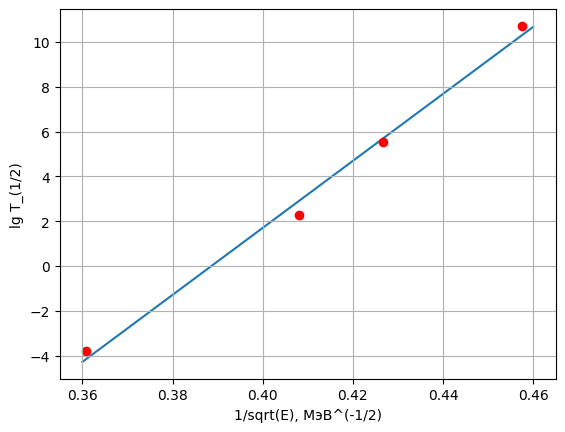
\includegraphics[width = 0.4\textwidth]{2.png}
  \end{center}
  \caption{Построение зон Френеля}
\end{wrapfigure}
Для выкладок ниже нам потребуется знать \textbf{принцип Гюйгенса-Френеля}. Он формулируется следующим образом:\\
\textbf{Каждый элемент волнового фронта можно рассматривать как центр  вторичного возмущения, порождающего вторичные сферические волны, а результирующее световое поле  в каждой точке пространства будет определяться интерференцией этих волн.}\\
Теперь рассмотрим первое применение этого принципа, получившее название \textit{метод зон Френеля}

\begin{wrapfigure}{r}{0.3\textwidth}
  \begin{center}
    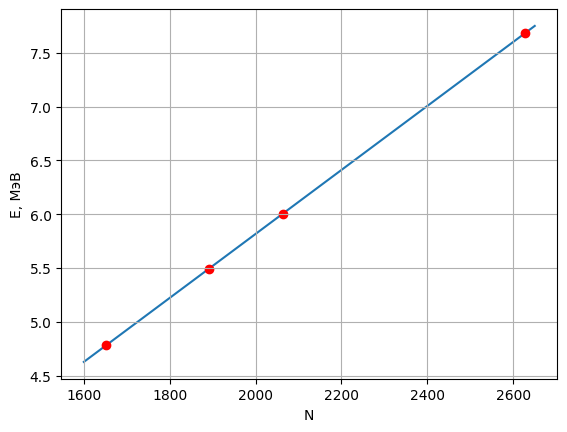
\includegraphics[width = 0.3\textwidth]{1.png}
  \end{center}
  \caption{К фазовым соотношениям при дифракции Фраунгофера}
  \vspace{+30pt}
\end{wrapfigure}

Для этого рассмотрим действие световой волны действующей из точки $A$ в какой-то точке $B$.
В этом случае можно, взяв точку $M_0$ в качестве центра (см. рис. 1), построить ряд концентрических сфер, радиусы которых начинаются с $b$ и увеличиваются каждый раз на половину длины волны $\frac{\lambda}{2}$. При пересечении с плоским фронтом волны $F$ эти сферы дадут концентрические окружности. Таким образом, на фронте волны появятся кольцевые зоны (зоны Френеля) с радиусами $r_1, r_2$ и т. д.

Из геометрических соображений посчитав, можно получить, что 
\begin{equation}
r_i = i \sqrt{a \lambda}
\end{equation}

Картина дифракции упрощается, когда ширина щели становится значительно меньше ширины первой зоны Френеля, т.е. если 
\begin{equation}
D \ll\sqrt{a \lambda} 
\end{equation}	
Это условие всегда выполняется при достаточно большом $a$. В этом случае говорят, что \textit{дифракция Фраунгофера}. Дифракционную картину в этом случае называются \textit{дифракцией Фраунгофера}. При выполнении пункта $(2)$ у нас упрощаются фазовые соотношения, что поясняет рис. 2, в итоге с хорошим приближением можно считать, что разность хода между крайними лучами, приходящими от щели в точке наблюдения $P$, с хорошим приближением равна 
\begin{equation}
\Delta = r_2 - r_1 \approx D \sin \theta \approx D \cdot \theta
\end{equation}
Здесь предполагается, что $\theta$ достаточно мал.
Дифракцию Фраунгофера можно наблюдать на установке Рис. 1, но для удобства к подобной установке добавляется объектив $O_2$.

\begin{figure}[h]
\includegraphics[width = 0.7\textwidth]{3.png}
\centering
\caption{Схема установки 2.}
\end{figure}
Дифракционная картина здесь наблюдается в фокальной плоскости объектива $O_2$. Каждому значению $\theta$ соответствует в этой плоскости точка, отстоящая от оптической оси на расстоянии 
\begin{equation}
X = f_2 \tan \theta \approx f_2 \theta.
\end{equation}
Объектив не вносит разности хода между интерферирующими лучам, поэтому в его фокальной плоскости наблюдается неискажённая дифракционная картина. При $\theta = 0$ разность хода между лучами нулевая, поэтому в центре поля зрения дифракционный максимум. Первый минимум соответствует $\theta_1$ такому, что в точке наблюдения разность хода пробегаем все значения от 0 до $2\pi$. Аналогично рассуждая, для $m$-й полосы
\begin{equation}
\theta_m = \frac{m \lambda}{D}
\end{equation}
Расстояние $X_m$ тёмной полосы от оптической оси из (5) и (6)
\begin{equation}
x_m = f_2m\frac{\lambda}{b}
\end{equation}

\section{Практическая часть}
\subsection{Дифракция Френеля}
Соберем установку на рис. 1. Для этого включим ртутную лампу и поставим после нее фильтр с щелью. После щели нужно будет поставить линзу так, чтобы щель была в фокусе. Для этого воспользуемся зрительной трубой, настроенной на бесконечность. Поскольку, если линза находится в нужном месте, из нее выходит пучок параллельных лучей, зрительная труба, настроенная на бесконечность, должна показать четкое изображение щели. После установки линзы поместим щель $S_2$ и микроскоп после неё.
Найдем нуль микрометрического винта щели $S_2$. Для этого посмотрим свозь щель на лампу накаливания и начнем поворачивать винт из нулевого положения до тех пор, пока свет от лампы не станет виден. При этом положение винта будет нулем.

\begin{center}
\begin{tabular}{|c|c|c|c|}
\hline
$d, \text{мкм}$&$57$&$56$&$56$\\ \hline
\end{tabular}\\~\\
\end{center} 
\[<d> = 56.3 \pm 1.0\; \text{мкм}\]

Измерим положение микроскопа $x$, при котором видно $n$ полос и найдем расстояние $a$ до плоскостии наблюдения, которое равно смещению относительно положения $x_0=88.0\pm0.5\,\text{мм}$

\begin{table}[H]
\begin{center}
\begin{tabular}{|c|c|c|c|c|c|}\hline
$m$ & $x_{min}\text{, \text{мм}}$ & $x_{max}\text{, \text{мм}}$ & $ a\text{, \text{мм}}$&$\Delta a\text{, \text{мм}}$&$2\xi \text{, \text{мм}}$\\\hline
$1$ & $56.0$ & $54.0$ & $2$ &$0.1$&$0.11$\\\hline
$2$ & $50.5$ & $48.0$ & $2.5$ &$0.1$&$0.165$\\\hline
$3$ & $44.5$ & $43.0$ & $1.5$ &$0.1$&$0.15$\\\hline
$4$ & $41.0$ & $40.5$ & $0.5$ &$0.1$&$0.1$\\\hline
$5$ & $39.5$ & $38.5$ & $1.0$ &$0.1$&$0.15$\\\hline
\end{tabular}\\~\\
\end{center}
\caption{\label{tab:first}}
\end{table}

Ширина щели: $b = (0.15 \pm 0.05)\; \text{мм}$

\begin{figure}[H]
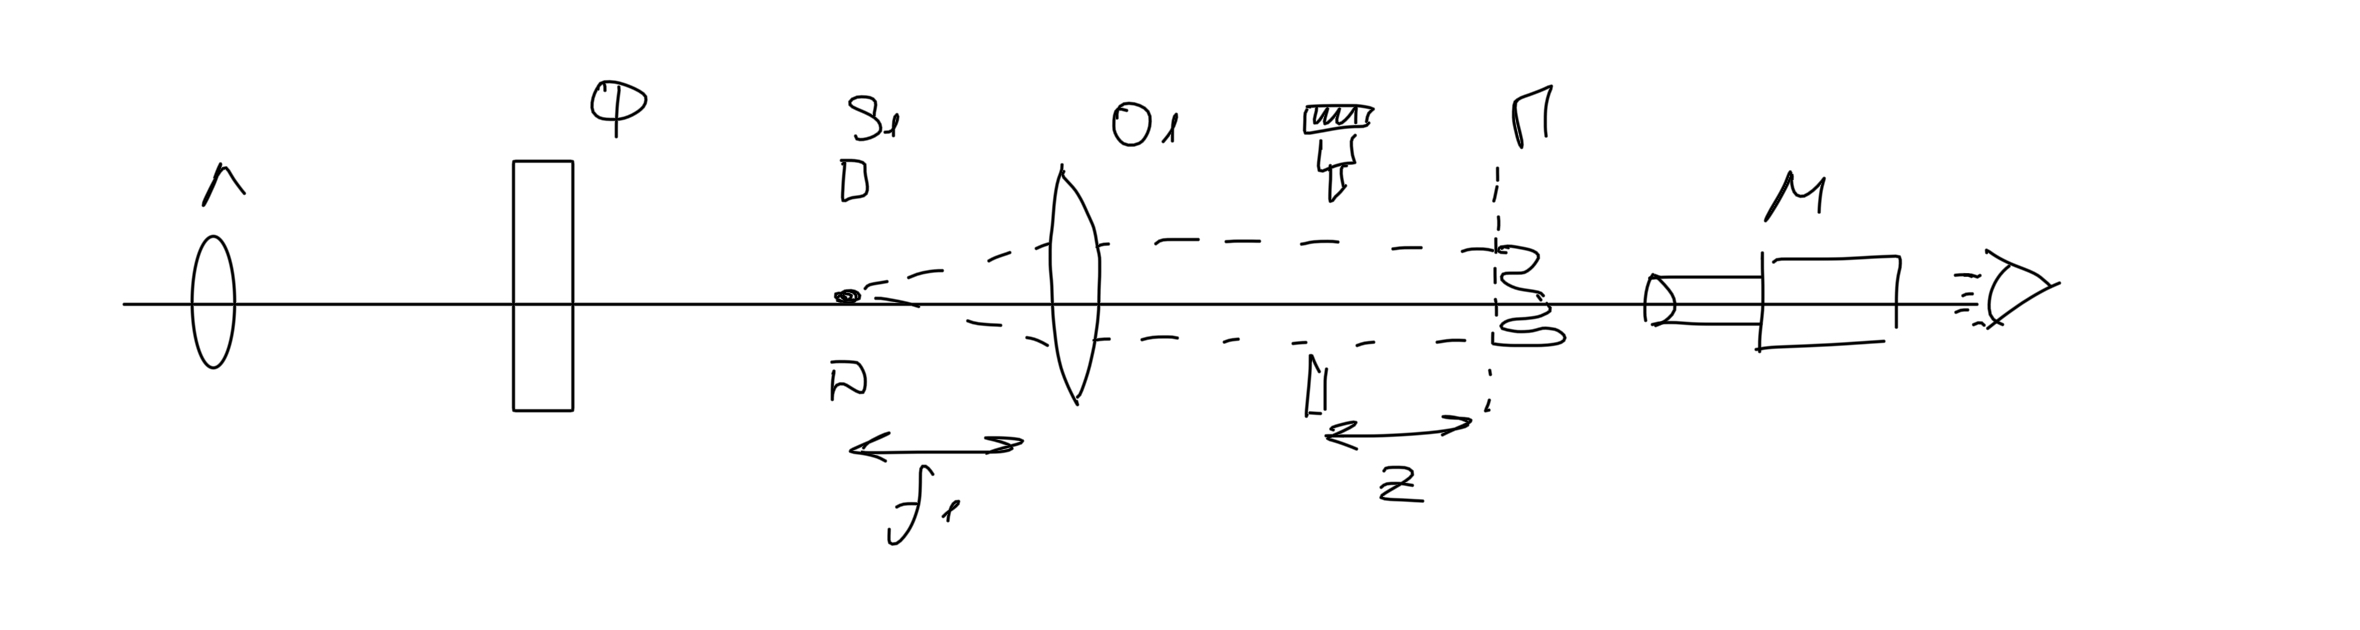
\includegraphics[scale=0.9]{frenel.png}
\end{figure}

Все результаты повторно сравниваются в выводах лабораторной работы.

\subsection{Дифракция Фраунгофера}

Фокусные расстояния линз: $F_1 = 11.5$ и $F_2 = 12.5$.

Ширина щели: $b = (0.303 \pm 0.05) \text{мм}$

Цена деления: 0.02 мм

Возьмём половину дифракционной картины Фраунгофера, так как можно получить данные до 6 порядка включительно (вторая половина аналогична). Рассчитаем также ширину щели по формуле (7):

\begin{table}[H]
\begin{center}
\begin{tabular}{|c|c|c|c|c|c|}\hline
$m$ & $Divisions$ & $x_m, \text{мм}$ & $\sigma(x_m), \text{мм}$ & $b, \text{мм}$ & $\sigma(b), \text{мм}$\\\hline
$1$ & $11$  & $0.22$ & $0.01$ & $ 0.310$ & 0.02\\\hline
$2$ & $23.5$ & $0.47$ & $0.01$ & $0.291$ & 0.02\\\hline
$3$ & $35.5$ & $0.71$ & $0.01$ & $0.288$ & 0.02\\\hline
$4$ & $47$ & $0.94$ & $0.01$ & $0.291$ & 0.02\\\hline
$5$ & $59$ & $1.18$ & $0.01$ & $0.289$ & 0.02\\\hline
$6$ & $68$ & $1.36$ & $0.01$ & $0.301$ & 0.02\\\hline
\end{tabular}\\~\\
\end{center}
\caption{\label{tab:second}}
\end{table}

Здесь расстояние $x_m$ - расстояние от оптической оси объектива до середины чёрной полосы.

Построим график зависимости этого расстояния от порядка $m$.

\begin{figure}[H]
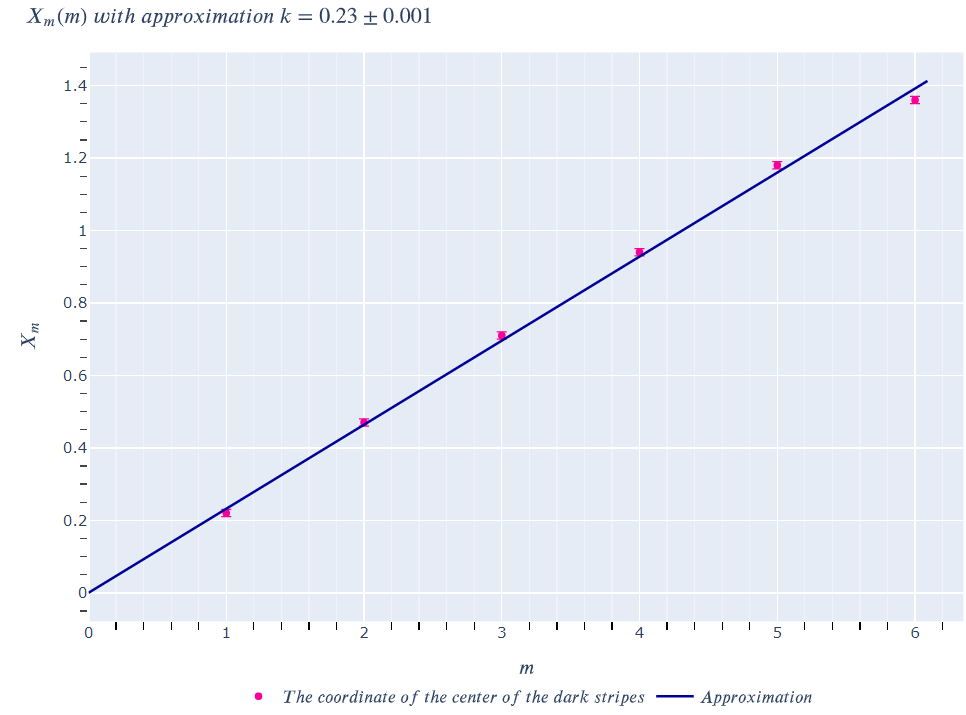
\includegraphics[scale=0.9]{Fraunhofer.png}
\end{figure}

Из графика  $k = 0.23$ - коэффициент наклона и есть $\Delta x$ - среднее расстояние между соседними минимумами.

Из Таблицы \ref{tab:second} $b_{\text{ср}} = 0.295\; \text{мм}$ 

Сделаем ещё один эксперимент с другой шириной щели, возьмём максимальную ширину щели $b = 4.0\; \text{мм}$

\begin{table}[H]
\begin{center}
\begin{tabular}{|c|c|c|c|c|c|}\hline
$m$ & $Divisions$ & $x_m, \text{мм}$ & $\sigma(x_m), \text{мм}$ & $b, \text{мм}$ & $\sigma(b), \text{мм}$\\\hline
$1$ & $9$  & $0.18$ & $0.01$ & $ 0.379$ & 0.02\\\hline
$2$ & $17$ & $0.34$ & $0.01$ & $0.402$ & 0.02\\\hline
$3$ & $27$ & $0.54$ & $0.01$ & $0.379$ & 0.02\\\hline
$4$ & $31.5$ & $0.63$ & $0.01$ & $0.433$ & 0.02\\\hline
$5$ & $41.5$ & $0.83$ & $0.01$ & $0.411$ & 0.02\\\hline
$6$ & $57.5$ & $1.15$ & $0.01$ & $0.356$ & 0.02\\\hline
$7$ & $72$ & $1.44$ & $0.01$ & $0.379$ & 0.02\\\hline
\end{tabular}\\~\\
\end{center}
\caption{\label{tab:third}}
\end{table}

\begin{figure}[H]
\includegraphics[scale=0.9]{Fraunhofer4.png}
\end{figure}

Из графика  $k = 0.19$ -  $\Delta x$ - среднее расстояние между соседними минимумами.

Из Таблицы \ref{tab:second} $b_{\text{ср}} = 0.391\; \text{мм}$ 


\subsection{Дифракция фраунгофера на 2-х щелях}

Измерим ширину главных максимума, посчитаем количество тёмных полос
\begin{equation*}
    X = (0.52 \pm 0.01)\; \text{мм}
\end{equation*}
\begin{equation*}
    n = 11
\end{equation*}
\begin{equation*}
    \delta x = \frac{X}{n}
\end{equation*}
\begin{equation*}
    \delta x = (0.047 \pm 0.001)\; \text{мм}
\end{equation*}

Тогда расстояние между щелями, считается по формуле (7):
\begin{equation*}
    d = (1.45 \pm 0.03)\; \text{мм}
\end{equation*}

Сравним результаты с теоретическими:
\begin{equation*}
    d = (1,00 \pm 0.01)\; \text{мм}
\end{equation*}
\begin{equation*}
    D = (0,180 \pm 0.01)\; \text{мм}
\end{equation*}

Тогда количество светлых полос по теории:
\begin{equation*}
    n = 11
\end{equation*}

\subsection{Влияние дифракции на разрешающую способность
оптического инструмента}
Подберём ширину щели так, чтобы изображения обеих щелей почти сливались, но всё-таки ещё воспринимались раздельно.
\begin{equation*}
    b = 0.284
\end{equation*}
Сравнивая с формулой для критерия Релея, имеем пропорциональность, соответсвенно дифракционные пятна различимы.


\subsection{Вывод} 
Про суть явления: реальных вторичных источников нет, это удобный способ восприятия. Все что видно в дифракции, связано исключительно с наличием вещества, первичное излучение взаимодействует с молекулами из которых состоят границы щели, оно начинает переизлучать, оно же идет в разные стороны и именно его мы и наблюдаем.

Приведём таблицу полученных экспериментальных данных:
\begin{center}
\begin{table}[h]
\begin{tabular}{|c|c|c|c|c|c|}
\hline
                & \begin{tabular}[c]{@{}c@{}}Дифракция \\ Френеля\end{tabular} & \begin{tabular}[c]{@{}c@{}}Дифракция \\ Фраунгофера\\ на одной щели (1)\end{tabular} & \begin{tabular}[c]{@{}c@{}}Дифракция \\ Фраунгофера\\ на одной щели (2)\end{tabular}   &             
                & \begin{tabular}[c]{@{}c@{}}Дифракция \\ Фраунгофера\\ на двух щелях\end{tabular} \\ \hline
$D_{theor}$, мм & $0,15\pm 0,01$                                                          & $0,303 \pm 0,01$ & $0,4 \pm 0,01$ & $d_{theor}$, мм & $1,00\pm0,01$\\ 
\hline
$D_{prac}$, мм  & $0,16\pm 0,03$                                                        & $0,295\pm 0,02$                                                                            &  $0,391 \pm 0,02$ & $d_{prac}$, мм  & $1,45\pm0,03$                                                                             \\ \hline
\end{tabular}
\end{table}
\end{center}
Для лучшего понимания, был сделан второй эксперимент с дифракцией Фраунгофера. Также приводится схематичный график сравнения интенсивностей:

\centering
\begin{figure}[H]
\includegraphics[scale=0.7]{intense.png}
\end{figure}
\centering

\end{document}
